\documentclass[problem]{mcs}

\begin{pcomments}
  \pcomment{PS_3color_crossover_SAT}
  \pcomment{by ARM 4/6/14}
\end{pcomments}

\pkeywords{
  coloring
  planar
  3-coloring
}

%%%%%%%%%%%%%%%%%%%%%%%%%%%%%%%%%%%%%%%%%%%%%%%%%%%%%%%%%%%%%%%%%%%%%
% Problem starts here
%%%%%%%%%%%%%%%%%%%%%%%%%%%%%%%%%%%%%%%%%%%%%%%%%%%%%%%%%%%%%%%%%%%%%

\begin{problem}
The 3-coloring problem for planar graphs turns out to be no easier
than the 3-coloring problem for arbitrary graphs.  This claim follows
very simply from the existence of a ``3-color cross-over gadget.''
Such a gadget is a planar graph whose outer face is a cycle with four
designated vertices $u,v,w,x$ occurring in clockwise order such that

\begin{itemize}
\item Any assignment of colors to vertices $u$ and $v$ can be
  completed into a 3-coloring of the gadget.
\item In every 3-coloring of the gadget, the colors of $u$ and $w$ are
  the same, and the colors of $v$ and $x$ are the also same.
\end{itemize}

So to find a 3-coloring for any simple graph, simply draw it in the
plane with edges crossing as needed, and then replace each occurrence
of an edge crossing by a copy of the gadget as shown in
Figure~\ref{fig:replace-crossing}.

\begin{figure}\inbook{[h]}
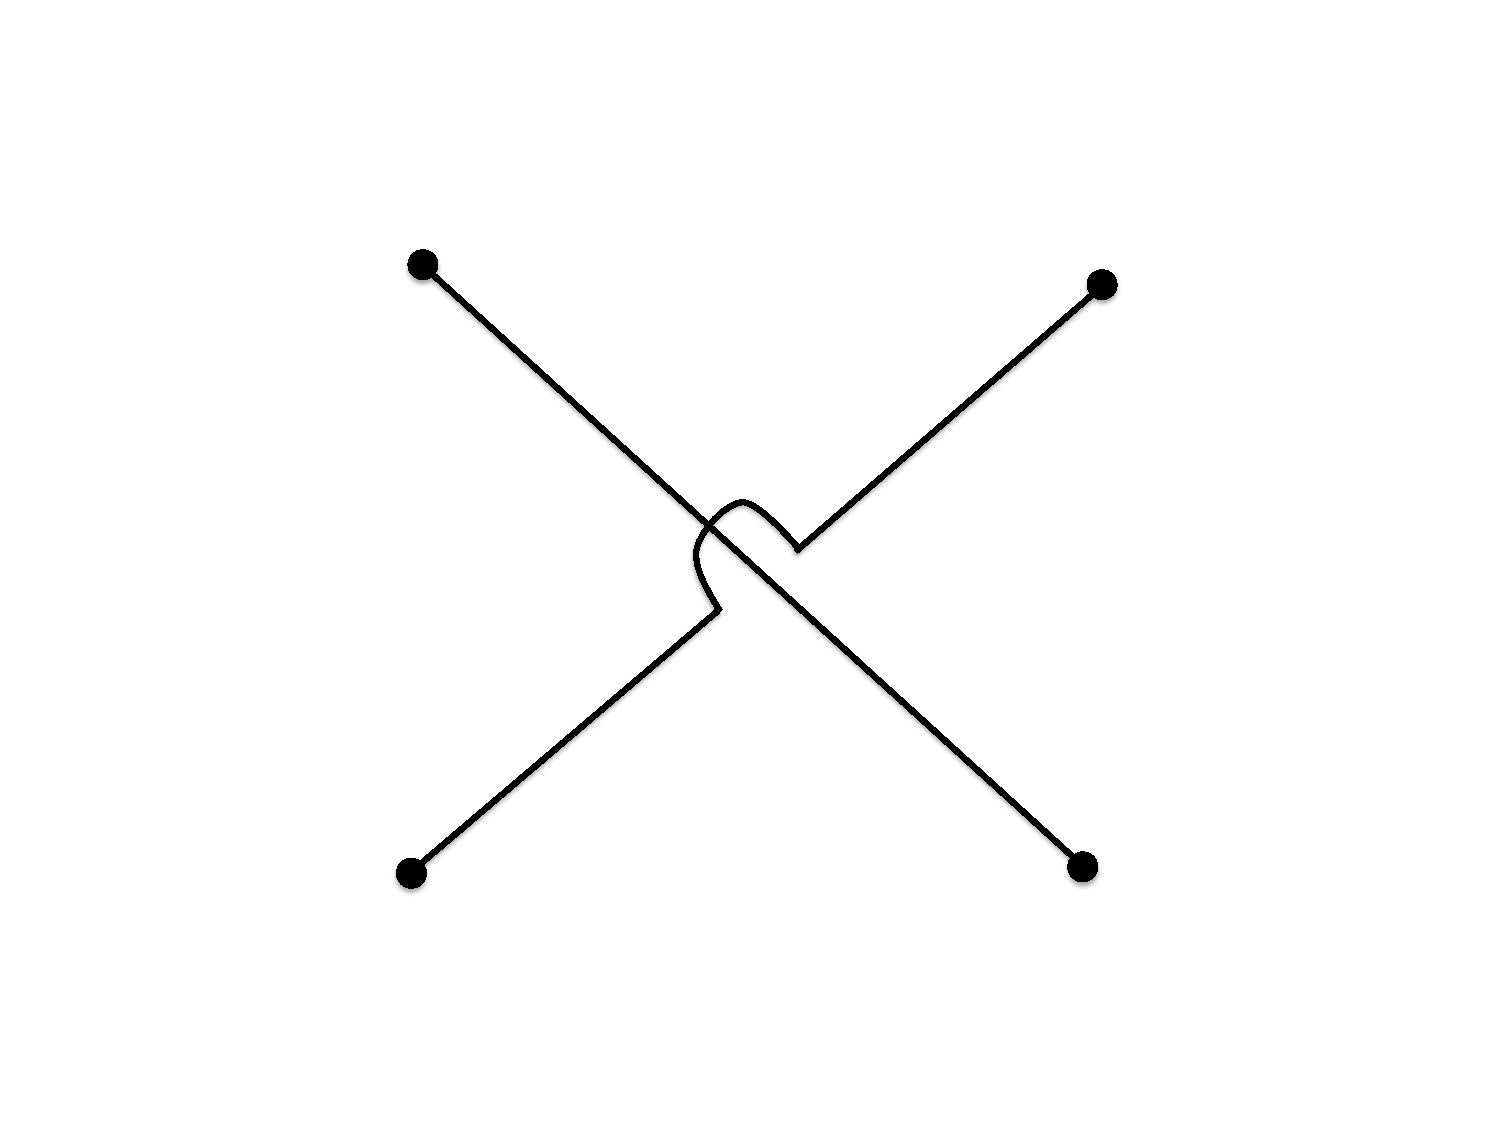
\includegraphics[width=2in]{edge-crossing} 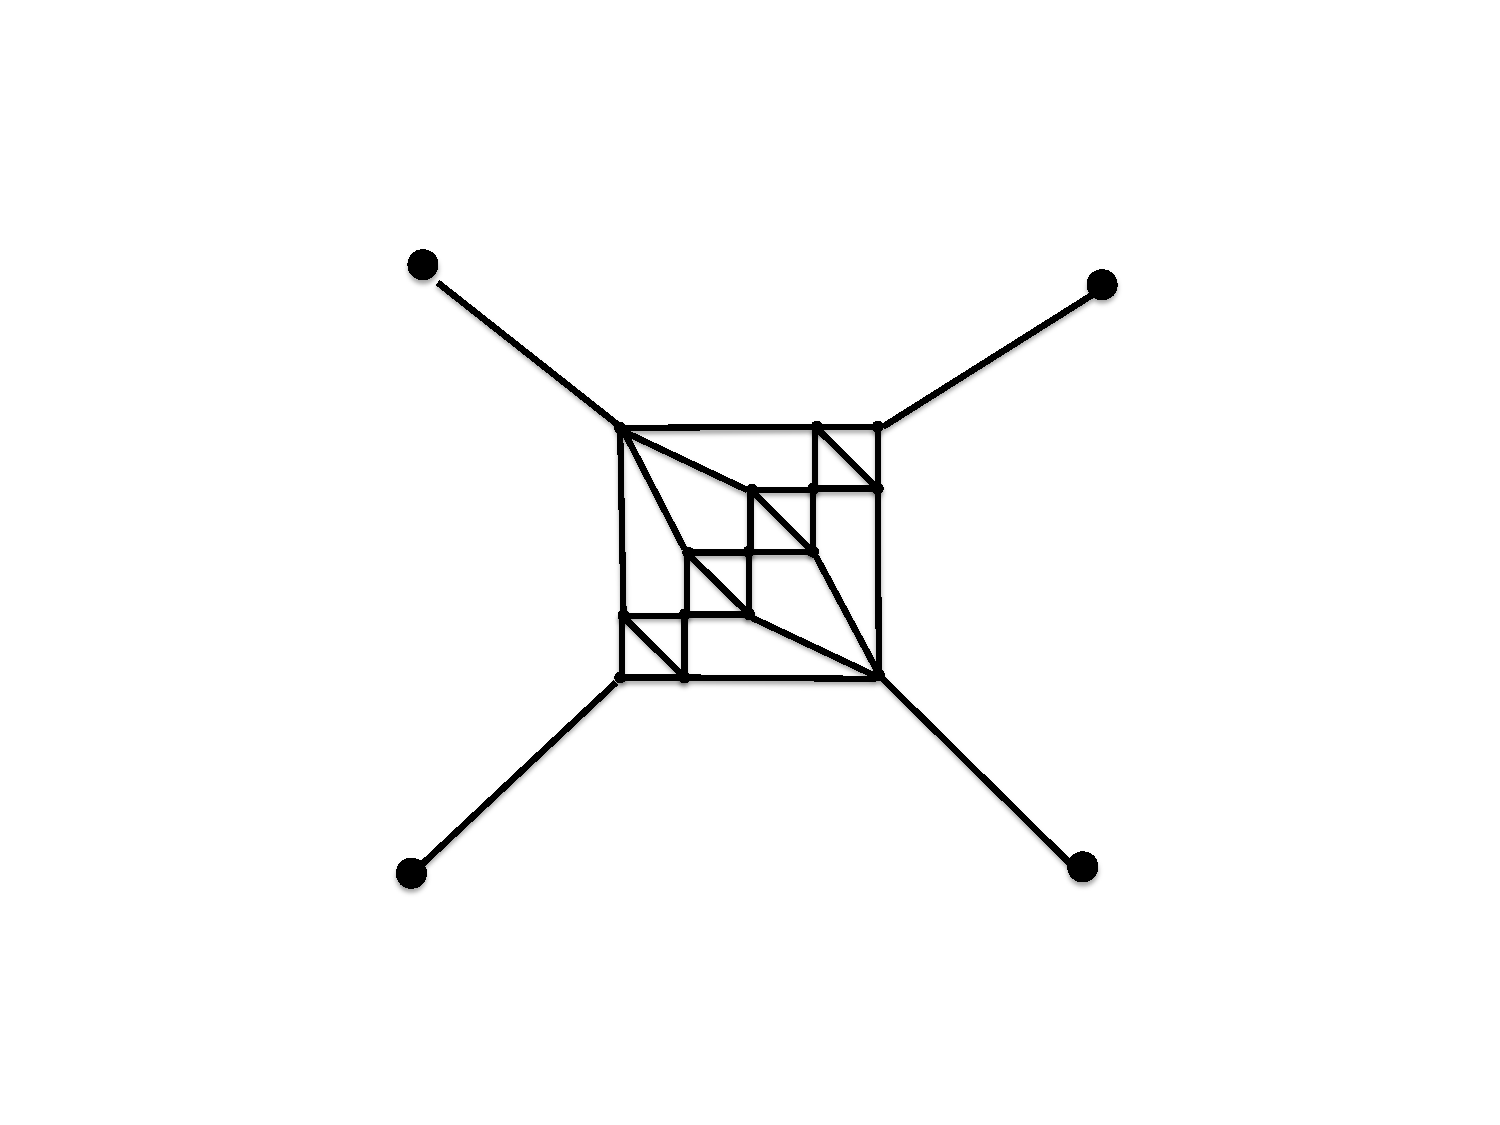
\includegraphics[width=2in]{3color-gadget-crossing}
\caption{Replacing an edge crossing with a planar gadget.}
\label{fig:replace-crossing}
\end{figure}

\end{problem}

%%%%%%%%%%%%%%%%%%%%%%%%%%%%%%%%%%%%%%%%%%%%%%%%%%%%%%%%%%%%%%%%%%%%%
% Problem ends here
%%%%%%%%%%%%%%%%%%%%%%%%%%%%%%%%%%%%%%%%%%%%%%%%%%%%%%%%%%%%%%%%%%%%%

\endinput
